\documentclass[11pt]{article}
\usepackage{graphicx}
\usepackage{color, soul}
\usepackage{amsmath}
\usepackage{systeme}
\usepackage{spalign}
\usepackage{listings}
\usepackage{nicefrac}
\usepackage{empheq}
\usepackage[most]{tcolorbox}

\title{\vspace{-3.0cm}Report for Benjamin}
\author{Riccardo Di Dio}
\date{\today}

\begin{document}
\maketitle
\section{RC model}
The schematic of the model can be seen in figure\ref{fig:LungModelRC}
where $V_g(t)$ represents the difference in pressure between athmosphere and pleural pressure while $i_0(t)$ is the respiratory flow. $R_0$ is the resistance of the trachea, $R_1$ and $R_2$ the resistances of the bifurcations. The resistances can be  gotten by Poiseuille: $R_i = \frac{8\eta L_i}{\pi r_i^4}$. $C_1$ and $C_2$ are the compliances of the 2 compartments.
\begin{figure}[ht]
\label{fig:LungModelRC}
\centering
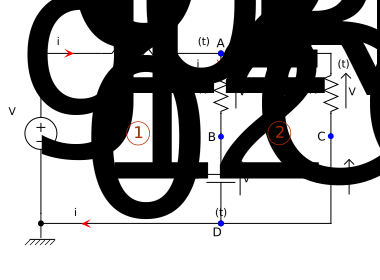
\includegraphics[scale=1.3]{LungModelRC.pdf}
\caption{Electrical equivalent of a bifurcation. 2 compartments are studied.}
\end{figure}
LKI equations:
\begin{equation}
\label{eq:LKI}
i_0(t) = i_1(t) + i_2(t)
\end{equation}
LKV equations:
\begin{equation}
\label{eq:LKV}
  \systeme*{
  	V_g(t) = V_0(t) + V_{R1}(t) + V_{C1}(t),
	V_g(t) = V_0(t) + V_{R2}(t) + V_{C2}(t)
  }
\end{equation}
Components:
\begin{equation}
\label{eq:components}
  \spalignsys{
  	i_{1}(t) = C_1\frac{dV_{C1}(t)}{dt};
	i_{1}(t) = \frac{V_{R1}(t)}{R_1};
  	i_{2}(t) = C_2\frac{dV_{C2}(t)}{dt};
	i_{2}(t) = \frac{V_{R2}(t)}{R_2};
  }
\end{equation}
So I can write:
\begin{equation}
\label{eq:dV/dt}
\spalignsys{
	\frac{dV_{C1}(t)}{dt} = \frac{V_{R1}(t)}{R_1C_1};
	\frac{dV_{C2}(t)}{dt} = \frac{V_{R2}(t)}{R_2C_2}
}
\end{equation}
Calling \hl{$\tau_1 = R_1C_1$} and \hl{$\tau_2 = R_2C_2$} and sobstituting \eqref{eq:dV/dt} in the LKV \eqref{eq:LKV}:
\begin{equation}
\label{eq:V_g(t)}
\spalignsys{
	V_g(t) = V_0(t) + \frac{dV_{C1}(t)}{dt}\tau_1 + V_{C1}(t);
	V_g(t) = V_0(t) + \frac{dV_{C2}(t)}{dt}\tau_2 + V_{C2}(t)
}
\end{equation}
which can be rewritten in canonic form as:
\begin{empheq}[box=\tcbhighmath]{equation}
\label{eq:ODE}
\spalignsys{
	\frac{dV_{C1}(t)}{dt} + \frac{1}{\tau_1}V_{C1}(t) = \frac{1}{\tau_1}(V_g(t) - V_0(t));
		\frac{dV_{C2}(t)}{dt} + \frac{1}{\tau_2}V_{C2}(t) = \frac{1}{\tau_2}(V_g(t) - V_0(t))
}
\end{empheq}
Equation \eqref{eq:ODE} represents the 2 ordinary differential equations got.

\section{Questions}
\begin{itemize}
\item \textit{Is this actually correct}?
\end{itemize}
Also now I have gotten these 2 ODE. I tried to combine them by using \eqref{eq:V_g(t)} 
\begin{equation}
\frac{dV_{C1}(t)}{dt}\tau_1 + V_{C1}(t) = \frac{dV_{C2}(t)}{dt}\tau_2 + V_{C2}(t)
\end{equation}
and then using the LKI \eqref{eq:LKI} where you can explicit the dipendence of $dV_{C1}/dt$ from $dV_{C2}/dt$ and $i_0$ explicitely. Moreover $i_0(t) = V_0(t)/R_0$. We get:\\
\begin{equation}
\begin{aligned}
	\frac{V_0(t)}{R_0} = C_1\frac{dV_{C1}(t)}{dt} + C_2\frac{dV_{C2}(t)}{dt}\\
	\Rightarrow V_0(t) = R_0C_1\frac{dV_{C1}(t)}{dt} + R_0C_2\frac{dV_{C2}(t)}{dt}
	\end{aligned}
\end{equation}
By sobstituting $V_0(t)$ in one of the 2 equations in \eqref{eq:ODE} we finally get:
\begin{empheq}[box = \tcbhighmath]{equation}
\label{eq:Final}
\spalignsys{
	\frac{dV_{C1}(t)}{dt} + \frac{1}{\tau_1}V_{C1}(t) = \frac{1}{\tau_1}(V_g(t) - V_0(t));
		\frac{dV_{C2}(t)}{dt} + \frac{1}{\tau_2}V_{C2}(t) = \frac{1}{\tau_2}(V_g(t) - V_0(t));
	V_0(t) = R_0C_1\frac{dV_{C1}(t)}{dt} + R_0C_2\frac{dV_{C2}(t)}{dt}
}
\end{empheq}
where the first 2 equations are from LKV and the last from LKI.\\
I'm not sure I can play with this system or if I'm actually missing something.
Indeed I suppose the following variables are known:
$$R_0,\hspace{2px}R_1,\hspace{2px}R_2,\hspace{2px}C_1,\hspace{2px}C_2,\hspace{2px}i_0(t)$$
Hence since $i_0(t)$ and $R_0$ are known, also $V_0(t)$ is known.\\
However the variables I don't know are:
$$V_{C1}, \hspace{2px}V_{C2}, \hspace{2px}\frac{dV_{C1(t)}}{dt}, \hspace{2px}\frac{dV_{C2(t)}}{dt}$$ 
I'm not too sure how to move from here.
\begin{itemize}
\item \textit{Can I suppose to know $V_g(t) - V_0(t)$}? This would be the difference in pressure between the nodes \textbf{A} and \textbf{D}, assuming the pleural pressure as reference $\rightarrow$ $V_D = 0$
\end{itemize}
\section{While waiting for the meeting}
I'll probably go ahead on math trying to get a proper system with a number of equation equal to the number of unknowns. I'm not sure I've already gotten it or not. Also I'm continuing to make myself a culture on lung modelling in literature and Pozin's thesis.
%\lstinputlisting[language = Python]{/home/rickyd/Documents/Work/LungModel/BronchoClass.py}
\end{document}